\documentclass{article}

\usepackage{apacite}
\usepackage{biblatex}
\usepackage{graphicx}

\bibliography{Citations}

\title{Maschinelles Lernen im Kontext der Programmierung natürlicher Sprachen}
\date{WS 18/19}
\author{Weinmann Philipp}

\begin{document}
\maketitle

\bibliographystyle(apacite)
\bibliography{References}

\newpage{}

\begin{figure}[h]
  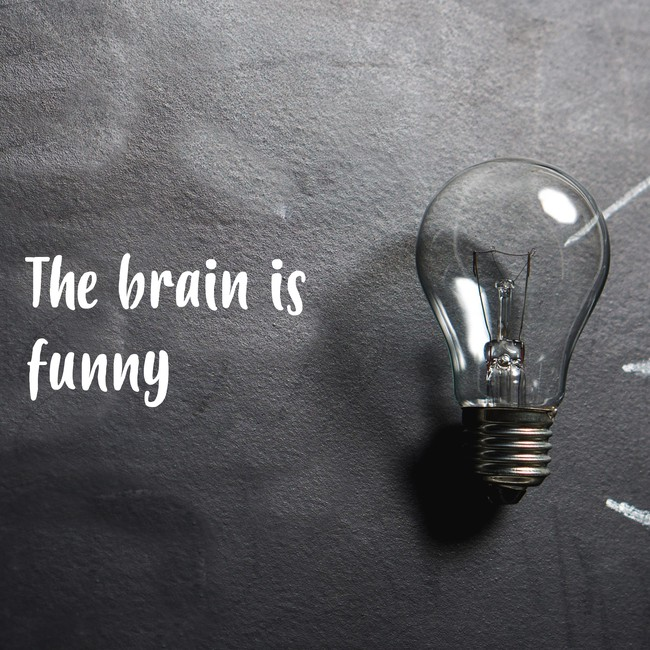
\includegraphics[width=\linewidth]{images/inspirobotQuote.jpg}
  \caption{quote generated through an AI}
  \label{fig:Inspirational quote by AI \cite{inspirobot}}
\end{figure}
\section{Was ist Maschinelles Lernen}
Teilbereich der KI. Benutzt unter anderem statistische Techniken um zu "lernen". Progressiv wird die effizienz eines Programms verbessert ohne das dieses explizit programmiert wird.
\section{Aufkommen von Maschinellem Lernen}
Kurze historische Zusammenfassung.
\section{Anwendungen im Bereich der Informatik	}
\begin{itemize}
	\item Klassifizierung
	\item Zusammenhänge erkennen
\end{itemize}
Diese Eigenschaften machen Maschine Learning zum perfekten Werkzeug für maschinelle Übersetzungen.
\section{Maschine Translation}
Die Anwendung von Software um Text von einer Sprache zur anderen zu übersetzen.
\subsection{Verschiedene methoden der Maschine Translation}
\begin{itemize}
	\item Regelbasiert
	\item Statistische Übersetzung
	\item Neuronale Maschinenübersetzung
\end{itemize}
\newpage
\section{Neuronale Maschinenübersetzung}
\subsection{Neuronale Netze, Einführung}
\begin{figure}[h]
  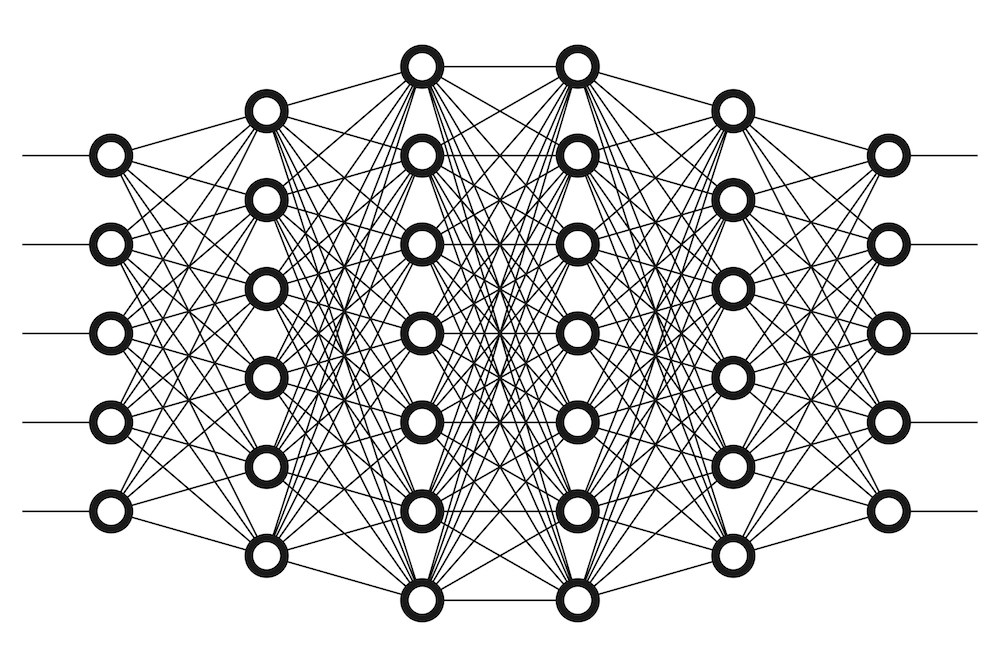
\includegraphics[width=\linewidth]{images/DeepNeuralNetwork.jpg}
  \caption{https://machine-learning-blog.de/2017/11/02/was-ist-deep-learning/}
  \label{fig:Neuronales Netz}
\end{figure}
\subsection{In der Industrie}
\begin{itemize}
	\item Google
	\item Microsoft
	\item Yahoo
\end{itemize}
\subsection{Kuriositäten}
\begin{itemize}
	\item Facebook chatbots haben eine eigene Sprache erfinden um zu kommunizieren.
	\item Google Translate hat eine Sprache erfunden die als Zwischensprache dient.
\end{itemize}
Fazit: Es ist schwer bzw unmöglich die Funktionsweise von Programmen die anhand von NN netzen entstanden sind zu verstehen oder zu kontrollieren.
\section{Bewertung}
	
\end{document}
